\section{Integrating Mathematical Software Systems via the Math-in-the-Middle Approach}

% Mathematics has a rich notion of data: it can be either numeric or symbolic data;
% knowledge about mathematical objects given as statements (definitions, theorems or
% proofs); or software that computes with these mathematical objects. All this data is
% really a common resource, and should be maintained as such


To achieve the goal of assembling the ecosystem of mathematical software systems in the
\pn project into a coherent mathematical VRE, we have to make the systems interoperable at
a mathematical level. In particular, we have to establish a common meaning space that
allows to share computation, visualization of the mathematical concepts, objects, and
models (COMs) between the respective systems. Building on this we can build a VRE with
classical IDE techniques. 

Concretely, the problem is that the software systems in \pn have their own representations
of and functionalities for the COMs involved. This starts with simple naming issues (e.g.\
elliptic curves are named \lstinline|ec| in the \LMFDB, and as \lstinline|EllipticCurve|
4bin \Sage), persists through the underlying data structures (five-tuple of natural numbers
for the Weierstrass equation in the \LMFDB and \ednote{MK: how in \Sage? Find a system
  where this is really different}), and becomes virulent at the level of algorithms, their
parameters, and domains of applicability.

To obtain a common meaning space for a VRE, we have the three well-known approaches in
Figure~\ref{fig:interop}
\begin{figure}[ht]\centering
  \begin{tabular}{|c|c|c|}\hline
    peer to peer & open standard & industry standard\\\hline
    \documentclass{standalone}
\usepackage{tikz}
\begin{document}
    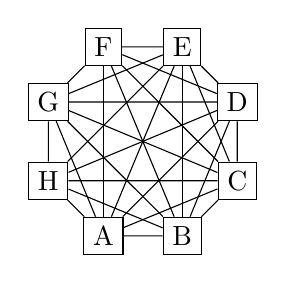
\begin{tikzpicture}
      \node[draw] (a) at (0,.3) {A};
      \node[draw] (b) at (1,.3) {B};
      \node[draw] (c) at (1.7,1) {C};
      \node[draw] (d) at (1.7,2) {D};
      \node[draw] (e) at (1,2.7) {E};
      \node[draw] (f) at (0,2.7) {F};
      \node[draw] (g) at (-.7,2) {G};
      \node[draw] (h) at (-.7,1) {H};
      \draw (a) -- (b) -- (c) -- (d) -- (e) -- (f) -- (g) -- (h) -- (a);
      \draw (a) -- (c) -- (h) -- (d) -- (g) -- (e);
      \draw (b) -- (h);
      \draw (b) -- (f);
      \draw (b) -- (d);
      \draw (b) -- (g);
      \draw (b) -- (e);
      \draw (h) -- (e);
      \draw (d) -- (f);
      \draw (g) -- (c);
      \draw (a) -- (d);
      \draw (a) -- (e);
      \draw (a) -- (f);
      \draw (a) -- (g);
      \draw (e) -- (c);
      \draw (c) -- (f);
    \end{tikzpicture}
\end{document}
%%% Local Variables: 
%%% mode: latex
%%% TeX-master: t
%%% End: 
 & \documentclass{standalone}
\usepackage{tikz}
\begin{document}
    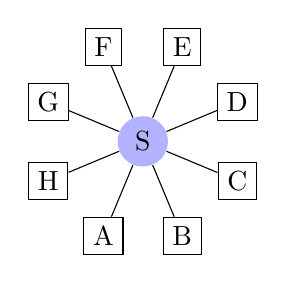
\begin{tikzpicture}
      \node[draw] (a) at (0,.3) {A};
      \node[draw] (b) at (1,.3) {B};
      \node[draw] (c) at (1.7,1) {C};
      \node[draw] (d) at (1.7,2) {D};
      \node[draw] (e) at (1,2.7) {E};
      \node[draw] (f) at (0,2.7) {F};
      \node[draw] (g) at (-.7,2) {G};
      \node[draw] (h) at (-.7,1) {H};
      \node[circle,fill=blue!30] (m) at (.5,1.5) {S};
      \draw (m) -- (a);
      \draw (m) -- (b);
      \draw (m) -- (c);
      \draw (m) -- (d);
      \draw (m) -- (e);
      \draw (m) -- (f);
      \draw (m) -- (g);
      \draw (m) -- (h);
    \end{tikzpicture}
\end{document}
%%% Local Variables: 
%%% mode: latex
%%% TeX-master: t
%%% End: 
 & \documentclass{standalone}
\usepackage{tikz}
\begin{document}
    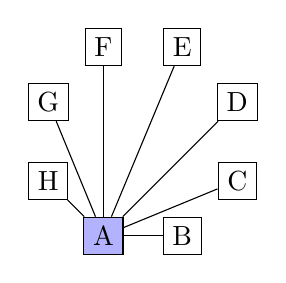
\begin{tikzpicture}
      \node[draw,fill=blue!30] (a) at (0,.3) {A};
      \node[draw] (b) at (1,.3) {B};
      \node[draw] (c) at (1.7,1) {C};
      \node[draw] (d) at (1.7,2) {D};
      \node[draw] (e) at (1,2.7) {E};
      \node[draw] (f) at (0,2.7) {F};
      \node[draw] (g) at (-.7,2) {G};
      \node[draw] (h) at (-.7,1) {H};
      \draw (a) -- (b);
      \draw (a) -- (c);
      \draw (a) -- (d);
      \draw (a) -- (e);
      \draw (a) -- (f);
      \draw (a) -- (g);
      \draw (a) -- (h);
    \end{tikzpicture}
\end{document}
%%% Local Variables: 
%%% mode: latex
%%% TeX-master: t
%%% End: 
\\\hline
    $n^2/2$  translations & $2n$ translations & $2n-2$ translations \\
    symmetric & symmetric & asymmetric\\\hline
  \end{tabular}
  \caption{Three Approaches for Safe Distributed Computation/Storage/UIs}\label{fig:interop}
\end{figure}
The first does not scale to a project with about a dozen systems, for the third there is
no obvious contender in the \ODK ecosystem. Fortunatly, we already have a ``standard'' for
expressing the meaning of COMs -- \defemph{mathematical vernacular}: the language of
mathematical communication, and in fact all the COMs supported the \ODK VRE are documented
in mathematical vernacular in journal articles, manuals, etc.

The obvious problem is that mathematical vernacular is too 
\begin{inparaenum}[\em i\rm)]
\item \emph{ambiguous}: we need a human to understand structure, words, and symbols
\item \emph{redundant}: every paper introduces slightly different notions. 
\end{inparaenum}
Therefore we adopt an approach, where we partially formalize (\defemph{flexiformalize})
mathematical vernacular to obtain a flexiformal ontology of mathematics that can serve as
\ednote{MK: continue, essentially the St.\ Andrews stuff}

%%% Local Variables:
%%% mode: latex
%%% TeX-master: "paper"
%%% End:

%  LocalWords:  pn visualization lstinline ec lstinline Weierstrass ednote
